\section{Slučajevi upotrebe}
\subsection{Upravljanje nalozima}
\subsubsection{Registracija korisnika na sajtu restorana}
\begin{itemize}
    \item \textbf{Kratak opis}:
    Korisnik prvi put pristupa nalogu restorana i zato je neophodna registracija kako bi mogao poručiti hranu.
    \item \textbf{Učesnici}:
    Korisnik
    \item \textbf{Preduslovi}:
    Nema preduslova. 
    \item \textbf{Postuslovi}:
    Korisnik je registrovan. 
    \item \textbf{Glavni tok}:
   \begin{enumerate}
        \item Korisnik odlazi na nalog restorana i otvara formu za registraciju
        \item Korisnik popunjava formu za registraciju
        \item Sistem vrši validaciju registracije
        \item Sistem beleži novog korisnika u bazi
        \item Sistem obaveštava korisnika o uspešnosti registracije
\end{enumerate}
\end{itemize}
\begin {itemize}
\item \textbf {Alternativni tokovi}: 
 3a: Korisnik nije uneo ispravne podatke za registraciju.\\
 Slučaj upotrebe se nastavlja na koraku 2.
 \end{itemize}
 \begin{itemize} 
     \item \textbf{Dodatne informacije}
 \begin{itemize}
     \item Neophodni podaci za registraciju korisnika su validna e-mail adresa, ime, prezime, adresa, korisničko ime i lozinka.
    \item Sistem validira novog korisnika tako što proverava da li već postoji nalog sa unetom e-mail adresom. Neophodno je i da korisničko ime bude jedinstveno.
 \end{itemize}
 \end{itemize}
 
 \\
 \subsubsection{Kreiranje naloga za radnika upravo zaposlenog u restoranu}
\begin{itemize}
    \item \textbf{Kratak opis}:
   Radniku koji je upravo zaposlen u restoranu na poziciji koordinatora ili magacionera potrebno je napraviti nalog kako bi imao pristup sistemu.
    \item \textbf{Učesnici}:
    Menadžer, Koordinator, Magacioner
    \item \textbf{Preduslovi}:
    Magacioner/Koordinator je upravo dobio posao u restoranu.
    \item \textbf{Postuslovi}:
    Magacioner/Koordinator ima svoj nalog. 
    \item \textbf{Glavni tok}:
   \begin{enumerate}
        \item Menadžer odlazi na vebsajt i prijavljuje se unošenjem svog korisničkog imena i šifre
        \item Menadžer otvara formu za unošenje novog naloga za zaposlene
        \item Menadžer popunjava formu svim potrebnim podacima
        \item Menadžer potvrđuje unete podatke klikom na dugme 'Sačuvaj'
        \item Sistem beleži novog zaposlenog u bazi
        \item Sistem obaveštava Magacionera/Koordinatora o uspešnosti registracije slanjem e-mail poruke
\end{enumerate}
\end{itemize}
\begin {itemize}
\item \textbf {Alternativni tokovi}: 
 3a: Menadzer nije uneo ispravne podatke za registraciju.\\
 Slučaj upotrebe se nastavlja na koraku 2.
 \end{itemize}
 \begin{itemize} 
     \item \textbf{Dodatne informacije}
 \begin{itemize}
     \item Neophodni podaci za pravljenje naloga zaposlenom su validna e-mail adresa, ime, prezime, adresa, korisničko ime, lozinka, kao i odabir opcije da li je zaposleni, čiji je nalog u nastanku, koordinator ili magacioner.
    \item Sistem validira novog korisnika tako što proverava da li već postoji nalog sa unetom e-mail adresom. Neophodno je i da korisničko ime bude jedinstveno.
 \end{itemize}
 \end{itemize}

\subsection{Upravljanje porudžbinom}
Na slici je predstavljen opšti tok upravljanja porudžbinom. U zavisnosti od toga da li među zalihama ima dovoljno namirnica, porudžbina se prihvata ili odbija.

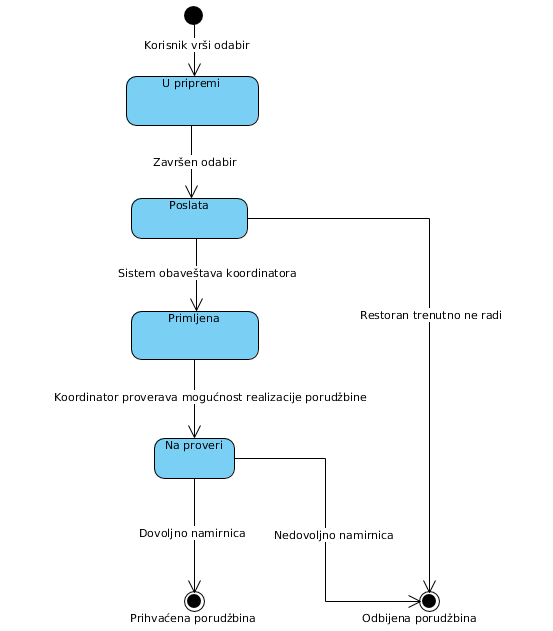
\includegraphics[width=136mm]{slike/Upravljanje_porudzbinom.png}\\
\begin{center}
\caption{Slika 3. Dijagram stanja}\\
\end{center}

 
 
\subsubsection{Onlajn naručivanje}
\begin{itemize}
    \item \textbf{Kratak opis}: Korisnik naručuje željenu hranu putem veb stranice. Porudžbina biva prihvaćena ili odbijena od strane koordinatora.
    \item \textbf{Učesnici}: Korisnik, koordinator.
    \item \textbf{Preduslovi}: Postojanje korisničkog naloga.
    \item \textbf{Postuslovi}: Prihvaćena, odnosno odbijena porudžbina.
    \item \textbf{Glavni tok}:
    
    1. Korisnik se prijavljuje na sajt restorana.\\
    2. Korisnik vrši odabir željenih proizvoda.\\
    3. Korisnik potvrđuje željenu porudžbinu klikom na dugme "Poruči".\\
    4. Sistem odbija porudžbinu u slučaju da restoran trenutno ne radi i obaveštava korisnika o tome.\\
    5. Sistem obaveštava koordinatora o prispeću zahteva.\\
    6. Koordinator proverava da li je moguće realizovati porudžbinu.\\
    7. Koordinator utvrđuje da svih namirnica potrebnih za datu porudžbinu ima u dovoljnim količinama.\\
    8. Koordinator prihvata porudžbinu klikom na dugme "Prihvati".\\
    9. Korisnik biva obavešten, od strane sistema, da je porudžbina prihvaćena.
    
     \item \textbf{Alternativni tokovi}:
     
     7. Koordinator utvrđuje da ne postoji dovoljna količina namirnica za pripremu porudžbine.\\
     8. Koordinator odbija porudžbinu klikom na dugme "Odbij".\\
     9. Korisnik biva obavešten, od strane sistema, da je porudžbina odbijena uz propratnu poruku.
    
\end{itemize}

\subsubsection{Naručivanje telefonom}
\begin{itemize}
    \item \textbf{Kratak opis}: Korisnik naručuje željenu hranu pozivom na telefon restorana. Porudžbina biva prihvaćena ili odbijena od strane koordinatora.
    \item \textbf{Učesnici}: Korisnik, koordinator.
    \item \textbf{Preduslovi}: Postojanje registrovanog telefonskog aparata u restoranu.
    \item \textbf{Postuslovi}: Prihvaćena, odnosno odbijena porudžbina.
     \item \textbf{Glavni tok}:
    
    1. Korisnik vrši poziv restorana.\\
    2. Korisnik vrši odabir željenih proizvoda.\\
    3. Koordinator proverava da li je moguće realizovati porudžbinu.\\
    4. Koordinator utvrđuje da svih namirnica potrebnih za datu porudžbinu ima u dovoljnim količinama.\\
    5. Koordinator prihvata porudžbinu i saopštava korisniku.\\
    6. Korisnik biva obavešten, od strane koordinatora, da je porudžbina prihvaćena.
    
    \item \textbf{Alternativni tokovi}:
     
     2. Korisnik biva obavešten, od strane telefonskog aprata, da restoran trenutno ne radi.\\
     4. Koordinator utvrđuje da ne postoji dovoljna količina namirnica za pripremu porudžbine.\\
     5. Koordinator odbija porudžbinu i saopštava korisniku.\\
     6. Korisnik biva obavešten, od strane koordinatora, da je porudžbina odbijena.
    
     
\end{itemize}


\subsection{Realizacija zahteva}
\subsubsection{Prosleđivanje porudžbine od koordinatora ka kuvaru}
\begin{itemize}
    \item \textbf{Kratak opis}:
    Koordinator prosledjuje zahtev za pripremu naručene hrane kuvaru.
    \item \textbf{Učesnici}:
    Koordinator, kuvar.
    \item \textbf{Preduslovi}:
    Postoje sve neophodne namirnice za pripremu poručenog jela.
    \item \textbf{Postuslovi}:
    Kuvar je primio zahtev za porudžbinom.
    \item \textbf{Glavni tok}:
   \begin{enumerate}
        \item Koordinator ostavlja cedulju sa naručenim jelom na glavni pult kuhinje. Cedulja sadrži i informaciju o adresi isporuke i ceni kao i podatak da li je porudžbina namenjena za ketering.
        \item Kooordinator usmeno obaveštava kuvara da postoji nova porudžbina.
        \item Kuvar preuzima cedulju sa informacijama o porudžbini.
\end{enumerate}
\end{itemize}

\subsubsection{Priprema naručenog jela}
\begin{itemize}
    \item \textbf{Kratak opis}:
    Kuvar priprema jelo koje je prethodno naručeno.
    \item \textbf{Učesnici}:
    Kuvar.
    \item \textbf{Preduslovi}:
    Nema preduslova.
    \item \textbf{Postuslovi}:
    Kuvar je pripremio jelo.
    \item \textbf{Glavni tok}:
   \begin{enumerate}
        \item Kuvar utvrđuje da li u kuhinji postoje sve namirnice koje
        su mu neophodne za pripremu porudžbine.
        \item Kuvar prikuplja namirnice koje će koristiti za pripremu hrane.
        \item Kuvar priprema naručenu hranu.
        \item Kuvar obaveštava koordinatora da je
        jelo pripremljeno.
\end{enumerate}
 \item \textbf{Alternativni tokovi}:\\
     1. Kuvar je utvrdio da u kuhinji ne postoje
     sve namirnice koje su neophodne.
     \\ Prelazi se na slučaj
    upotrebe "3.3.3 Donošenje namirnica koje nedostaju u kuhinji". Nakon završetka tog slučaja upotrebe
    vraća se na korak 2. 
\end{itemize}

\subsubsection{Donošenje namirnica koje nedostaju u kuhinji}
\begin{itemize}
    \item \textbf{Kratak opis}:
    Magacioner donosi u kuhinju namirnice koje su kuvaru potrebne za pripremu hrane.
    \item \textbf{Učesnici}:
    Magacioner, kuvar.
    \item \textbf{Preduslovi}:
    Nema preduslova.
    \item \textbf{Postuslovi}:
    Kuvar ima u kuhinji sve namirnice koje su mu potrebne za pripremu jela koje je poručeno.
    \item \textbf{Glavni tok}:
   \begin{enumerate}
        \item Kuvar poziva magacionera i zahteva iz magacina namirnice koje mu nedostaju.
        \item Magacioner prikuplja tražene namirnice.
        \item Magacioner donosi u kuhinju namirnice.
\end{enumerate}
\end{itemize}

\subsubsection{Prosleđivanje dekorateru porudžbine koju je potrebno aranžirati}
\begin{itemize}
    \item \textbf{Kratak opis}:
    Dekorater aranžira hranu koja je
    namenjena za ketering.
    \item \textbf{Učesnici}: 
    Dekorater, koordinator, kuvar.
    \item \textbf{Preduslovi}:
    Porudžbina je pripremljena i spremna
    za aranžiranje.
    \item \textbf{Postuslovi}:
    Dekorater je aranžirao ketering.
    \item \textbf{Glavni tok}:
   \begin{enumerate}
        \item Kuvar obaveštava koordinatora da
        je porudžbina pripremljena i može da 
        se aranžira.
        \item Kooordinator obaveštava
        dekoratera da postoji porudžbina koju je potrebno aranžirati.
        \item Dekorater preuzima porudžbinu i aranžira je.
        \item Dekorater javlja koordinatoru da 
        je porudžbina dekorisana i spremna za isporuku.
\end{enumerate}
\end{itemize}


\subsubsection{Preuzimanje porudžbine radi isporuke}
\begin{itemize}
    \item \textbf{Kratak opis}:
    Dostavljač preuzima iz kuhinje paket koji je potrebno isporučiti na adresu korisnika.
    \item \textbf{Učesnici}: 
    Koordinator, dostavljač.
    \item \textbf{Preduslovi}:
    Porudžbina je već pripremljena i aranžirana ukoliko je postojao zahtev za aranžmanom.
    \item \textbf{Postuslovi}:
    Dostavljač je primio paket koji treba isporučiti.
    \item \textbf{Glavni tok}:
   \begin{enumerate}
        \item Kooordinator obaveštava
        dostavljača da postoji porudžbina koju 
        treba da dostavi.
        \item Dostavljač preuzima iz kuhinje paket koji treba isporučiti zajedno sa ceduljom na kojoj se nalazi informacija o adresi isporuke i ceni.
        \item Dostavljač odlazi na adresu dostave radi isporuke porudžbine.
\end{enumerate}
\end{itemize}
 
